%%%%%%%%%%%%%%%%%%%%%%%%%%%%%%%%%%%%%%%%%%%%%%%%%%%%%%%%%%%%%%%%%%%%%%%%%%%%%%%%
%2345678901234567890123456789012345678901234567890123456789012345678901234567890
%        1         2         3         4         5         6         7         8

\documentclass[letterpaper, 10 pt, conference]{ieeeconf}  % Comment this line out
                                                          % if you need a4paper
%\documentclass[a4paper, 10pt, conference]{ieeeconf}      % Use this line for a4 paper
\IEEEoverridecommandlockouts                              % This command is only needed if you want to use the \thanks command
\overrideIEEEmargins
% See the \addtolength command later in the file to balance the column lengths on the last page of the document

% The following packages can be found on http:\\www.ctan.org
\usepackage{tikz}     % For adding axes to plots
\usepackage{graphicx} % For including PDFs
\usetikzlibrary{positioning}

%% \usepackage{graphics} % for pdf, bitmapped graphics files
%\usepackage{epsfig} % for postscript graphics files
%\usepackage{mathptmx} % assumes new font selection scheme installed
%\usepackage{times} % assumes new font selection scheme installed
\usepackage{amsmath} % assumes amsmath package installed
\usepackage{amssymb}  % assumes amsmath package installed

%% Command for creating multiplie-line cells inside a table environment
\newcommand{\multilinecell}[2][c]{%
  \begin{tabular}[#1]{@{}c@{}}#2\end{tabular}}


\title{\LARGE \bf Nonparametric Distribution Models for Predicting and
  \\ Managing Computational Performance Variability* }

\author{Thomas C. H. Lux$^{1}$, Layne Watson$^{2}$, Jon Bernard$^{1}$, Tyler H. Chang$^{1}$, Bo Li$^{1}$, \\ Li Xu$^{3}$, Godmar Back$^{2}$, Ali R. Butt$^{2}$, Kirk W. Cameron$^{2}$, Yili Hong$^{4}$% <-this % stops a space
\thanks{*This work was supported by the National Science Foundation}%
\thanks{$^{1}$T. Lux, J. Bernard, T. Chang, B. Li are doctoral students of Computer Science at Virginia Polytechnic Institute and State University, Blacksburg, Virginia 24060, USA {\tt\small (tchlux at vt.edu)}}%
\thanks{$^{2}$L. Watson, G. Back, A. Butt, and K. Cameron are Faculty of Computer Science at Virginia Polytechnic Institute and State University, Blacksburg, Virginia 24060, USA}%
\thanks{$^{3}$L. Xu is a doctoral student of Statistics at Virginia Polytechnic Institute and State University, Blacksburg, Virginia 24060, USA}%
\thanks{$^{4}$Y. Hong is with the Faculty of Statistics at Virginia Polytechnic Institute and State University, Blacksburg, Virginia 24060, USA}%
}

\begin{document}

\maketitle
\thispagestyle{empty}
\pagestyle{empty}

%%%%%%%%%%%%%%%%%%%%%%%%%%%%%%%%%%%%%%%%%%%%%%%%%%%%%%%%%%%%%%%%%%%%%%%%%%%%%%%%
\begin{abstract}
Performance variability can have a significant impact on many applications of computing. Cloud Computing, High Performance Computing, and Computer Security communities each exert considerable effort managing and analyzing variability throughout the system stack. This work presents and evaluates a methodology for predicting precise characteristics of the computational performance variability of an input/output (I/O) application over varying system configurations. Results demonstrate that the presented methodology is capable of precisely modeling performance variability, which could allow applications that tighten service level agreements, maximize computational throughput, and obfuscate system configurations against malicious users.
\end{abstract}
%%%%%%%%%%%%%%%%%%%%%%%%%%%%%%%%%%%%%%%%%%%%%%%%%%%%%%%%%%%%%%%%%%%%%%%%%%%%%%%%

\section{INTRODUCTION}
\label{sec:introduction}

Computational variability presents itself in a variety of forms. Processes that are apparently identical in a cloud computing or high performance computing (HPC) environment may take different amounts of time to complete the same job. This variability can cause unintentional violations of service level agreements in cloud computing applications or indicate suboptimal performance in HPC applications. The sources of variability, however, are distributed throughout the system stack and often difficult to identify. The methodology presented in this work is applicable to modeling the expected variability of useful computer system performance metrics without any prior knowledge of system architecture. Some examples of interesting performance metrics that could be modeled with the techniques in this work include computational throughput, power consumption, processor idle time, number of context switches, and RAM usage, as well as any other ordinal performance metric.

Predicting performance variability in a computer system is a challenging problem that has primarily been attempted in one of two ways: (1) build a statistical model of the performance data collected by running experiments on the system at select settings, or (2) run artificial experiments using a simplified simulation of the target system to estimate architecture and application bottlenecks. In this paper, the proposed modeling techniques rest in the first category and they represent a notable increase in the ability to model precise characteristics of variability.

Many previous works attempting to model system performance have used simulated environments to estimate the performance of a system \cite{grobelny2007fase,wang2009simulation,wang2013towards}. Some refer to statistical models as being oversimplified and not capable of capturing the true complexity of the underlying system. This claim is partially correct, noting that a large portion of predictive statistical models rely on simplifying the machine to one or two parameters \cite{snavely2002framework,bailey2005performance,barker2009using,ye2010analyzing}. These limited statistical models have provided satisfactory performance in very narrow application settings. Many of the aforementioned statistical modeling techniques claim to generalize, while simultaneously requiring additional code annotations, hardware abstractions, or additional application level understandings in order to generate models. The approach presented here requires no modifications of the application, no architectural abstractions, nor any structural descriptions of the input data being modeled. The techniques used are purely mathematical and only need performance data as input.

Among the statistical models presented in prior works, \cite{bailey2005performance} specifically mentions that it is difficult for the simplified models to capture variability introduced by I/O. System variability in general has become a problem of increasing interest to the cloud and HPC systems communities, however most existing work has focused on operating system (OS) induced variability \cite{beckman2008benchmarking,de2007identifying}. The work that has focused on managing I/O variability does not use any sophisticated modeling techniques \cite{lofstead2010managing}.

This paper presents an application of advanced statistical modeling to the domain of computer system I/O throughput. The models are used to predict the cumulative distribution function (CDF) of the expected I/O throughput for a system at previously unseen configurations. The techniques in this paper can tractably model tens of interacting system parameters with tens of thousands of unique configurations.

Section \ref{sec:variability_modeling} details the mathematical techniques used to approximate variability, the chosen measurement of error, and an optimization strategy for improving model performance. Section \ref{sec:data} summarizes the data collection process as well as provides summary statistics of the data used for the case study. Section \ref{sec:results} presents the results of the I/O case study including analyses of approximation accuracy, model convergence, and system parameter importance. Section \ref{sec:discussion} discusses possible explanations for witnessed results, potential applications of the predictive methodology, and future improvements of the models.

%% ===================================================================
\section{VARIABILITY MODELING}
\label{sec:variability_modeling}

Performance and its variability can be summarized by a variety of statistics. Mean, range, standard deviation, variance, and interquartile range are a few summary statistics that describe performance and variability. However, the most precise characterization of any ordinal performance metric is the cumulative distribution function (CDF), or its derivative the probability density function (PDF). Previous techniques for predicting system performance have strictly modeled real-valued summary statistics because there exists a large base of mathematical techniques capable of approximating functions of the form $f: \mathbb{R}^d \rightarrow \mathbb{R}$. There is a smaller theoretical foundation for approximating functions of the form $f: \mathbb{R}^d \rightarrow g$ with $g: \mathbb{R} \rightarrow \mathbb{R}$. The latter is the approximation of functions.

A major hurdle when modeling functions such as the CDF or PDF, is that certain properties must be maintained in order for the functions to remain valid. It is necessary that a PDF $f: \mathbb{R} \rightarrow \mathbb{R}$ have the properties $f(x) > 0$ and $\int_{-\infty}^{\infty}f(x)dx = 1$. However, for a CDF $F: \mathbb{R} \rightarrow \mathbb{R}$ the properties are $F(x) \in [0,1]$ and $F'(x) \geq 0$. For the purpose of function approximation, the properties of the CDF are more straightforward to maintain. This work utilizes the fact that a convex combination of CDFs results in a valid CDF. Given $G(x) = \sum_{i}w_i F_i(x)$, $\sum_{i} w_i = 1$, $w_i \geq 0$, and each $F_i$ is a valid CDF, $G$ must also be a valid CDF. A demonstration of how this is applied can be seen in Figure \ref{fig:prediction_example}. Next, the three techniques used to model CDFs are summarized, a mechanism for identifying important features is proposed, and the error measure used throughout this work is presented. For each of the following, $n \in \mathcal{N}$ refers to the number of training samples (known system configurations), $d \in \mathcal{N}$ refers to the dimension of the data (ordinal system parameters), $x^{(i)} \in \mathbb{R}^d$ is a known system configuration with known CDF $F_{x^{(i)}}$, and $y \in \mathbb{R}^d$ refers to a previously unseen system configuration with CDF $F_y$.

%% ===================================================================
\subsection{Delaunay}
\label{sec:delaunay}

The Delaunay method of interpolation is a well studied geometric technique for producing an interpolant \cite{lee1980two}. The Delaunay triangulation of a set of data points into simplices is such that the sphere defined by the vertices of each simplex contains no data points in the sphere's interior. For a $d$-simplex S with vertices $x^{(0)}$, $x^{(1)}$, $\ldots$, $x^{(d)}$, and functions $F_{x^{(i)}}$, $i=0$, $\ldots$, $d$, $y$ is a unique convex combination of the vertices,

$$ y = \sum_{i=0}^{d} w_i x^{(i)}, \quad \sum_{i=0}^{d} w_i = 1, \quad w_i \geq 0, \quad i=0,\ldots,d, $$

and the Delaunay interpolant $F_y$ at $x$ is given by

$$ F_y = \sum_{i=0}^{d} w_i F_{x^{(i)}}. $$

\begin{figure}[htb]
  \begin{tikzpicture}
    \node (img)  {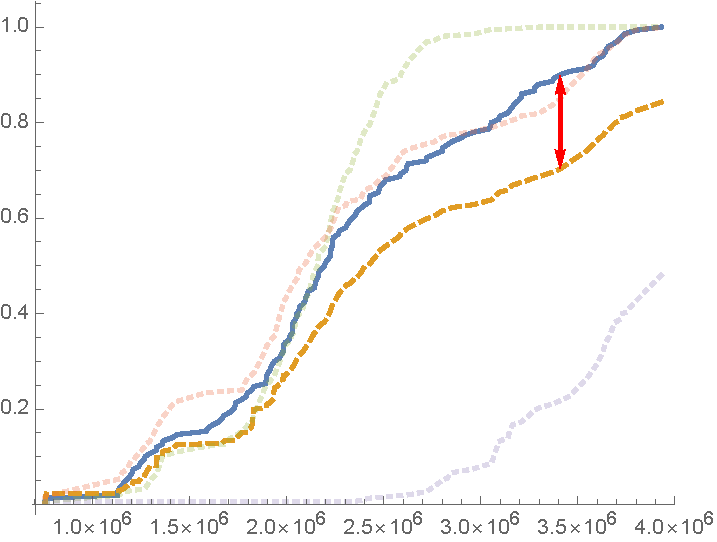
\includegraphics[width=0.4\textwidth,]{plot-delaunay-example-prediction.pdf}};
    \node[below=of img, node distance=1cm, yshift=1cm] {I/O Throughput};
    \node[left=of img, node distance=0cm, rotate=90, anchor=center,yshift=-0.7cm] {CDF Value};
  \end{tikzpicture}
  \vspace{-0.3cm}
  \caption{In this example, the general methodology for predicting a CDF and evaluating error can be seen. The Delaunay method chose three source system configurations (dotted lines) and assigned weights \{.3, .4, .3\} (top to bottom). The weighted sum of the three known CDFs produces the predicted CDF (dashed line). The KS Statistic (red arrow) computed between the true CDF (solid line) and predicted CDF (dashed line) is 0.2 for this example. This prediction is deemed a failure by p-values 0.05 and 0.01, however it is not a failure according to p-values 0.001 and 1.0e-6.
  \vspace{-.1cm}}
  \label{fig:prediction_example}
\end{figure}

The computational complexity of interpolating via Delaunay (for the implementation used) is approximately $\mathcal{O}(n d^4 log d)$, which is capable of scaling reasonably to $d \leq 50$. In the present application, Delaunay is used to select up to $d+1$ system configurations and assign weights to each in order to generate a prediction for a new system configuration.

%% ===================================================================
\subsection{Max Box Mesh}
\label{sec:max_box_mesh}

The Max Box mesh is an interpolation technique that utilizes overlapping box splines \cite{de2013box} as basis functions that are shifted and scaled to support box shaped regions. The boxes are constructed such that each box has strictly one point on its interior while maintaining the largest minimum distance between the interior point and the closest face of the box (a measure of centrality). Given a set of box splines $b^{x^{(i)}}$ with the max box properties anchored at each $x^{(i)}$,

$$ F_y = \frac{\sum_i b^{x^{(i)}}(y) F_{x^{(i)}}}{\sum_i b^{x^{(i)}}(y)}, $$

where $b^{x^{(i)}}(y) \geq 0$ and the denominator causes the sum of weights to be one. The computational complexity of interpolation via the Max Box mesh is $\mathcal{O}(n^2 d)$. The Max Box mesh interpolates a function $F_y$ by producing a convex combination of known functions $F_{x^{(i)}}$, where the weights are determined by the box splines.

%% ===================================================================
\subsection{Voronoi Mesh}
\label{sec:voronoi_mesh}

A well-studied technique for classification and approximation is the nearest neighbor algorithm \cite{cover1967nearest}. Nearest neighbor inherently utilizes the convex region surrounding a central control point in whose interior all points are closer to that center than any other control point, which is also called the Voronoi cell \cite{dirichlet1850reduction}. The Voronoi mesh smooths the nearest neighbor approximation by utilizing the Voronoi cells to define support via a generic basis function $v: \mathbb{R}^d \rightarrow \mathbb{R}_+$ with

$$ v^{x^{(i)}}(y) = \left(1 - \frac{||y - x^{(i)}||_2}{2 \ d(y - x^{(i)} \mid x^{(i)})} \right), $$

where $d(\ \cdot \mid x^{(i)})$ is the distance between $x^{(i)}$ and the nearest boundary of the Voronoi cell along the vector $\cdot\ $. While all basis functions $v^{x^{(i)}}(x^{(i)}) = 1$, the $2$ in the denominator causes all basis functions to go linearly to $0$ at the boundary of the twice-expanded Voronoi cell. Now we have

$$ F_y = \frac{\sum_i v^{x^{(i)}}(y) F_{x^{(i)}}}{\sum_i v^{x^{(i)}}(y)}, $$

where $v^{x^{(i)}}(y) \geq 0$ by definition and the denominator causes the sum of weights to be one. The computational complexity of interpolation via Voronoi mesh is $\mathcal{O}(n^2 d)$. The Voronoi mesh interpolates a function $F_y$ just as the Max Box mesh and Delaunay triangulation, by a convex combination of known functions $F_{x^{(i)}}$.
%% ===================================================================
\subsection{Feature Weighting}
\label{sec:feature_weighting}

Machine learning has demonstrated that an important procedure in any application of predictive methodologies is identifying those features of training data that are most relevant to making accurate predictions \cite{guyon2003introduction}. Selection strategies such as the floating searches studied in \cite{pudil1994floating} or others compared in \cite{ferri1994comparative} can be too expensive for large approximation problems. Rather, this work poses feature selection as a continuous optimization problem. Let $X$ be an $n \times d$ matrix of $n$ known system configurations with $d$ parameters each normalized to be in the unit cube. Define an error function $err: \mathbb{R}^d \rightarrow \mathbb{R}_+$ that estimates the error of a predictive model trained on $X diag(w)$, $w \in \mathbb{R}^d$,  by performing 10-fold cross validation using 80\% of the rows of $X diag(w)$ as training and 20\% as testing. A minimal solution to this error function could be considered an optimal weighting of the features of $X$. Minimization is performed using the modified simulated annealing technique presented in \cite{lux2016convergence} because of its empirically fast convergence in the absence of a readily computable gradient.

%% ===================================================================
\subsection{Measuring Error}

The performance of approximation techniques that predict functions can be analyzed through a variety of summary statistics. Mean error, mean absolute error, mean squared error, and the max absolute error are all popular measures. This work uses the max absolute error, also known as the Kolmogorov-Smirnov (KS) statistic \cite{lilliefors1967kolmogorov} for its compatibility with the KS test.

The two-sample KS test is a useful nonparametric test for declaring when two CDFs do not originate from the same underlying distribution while only assuming stationarity, finite mean, and finite variance. The null hypothesis (that two CDFs come from the same underlying distribution) is rejected at level $p \in [0,1]$ when

$$ KS > \sqrt{-\frac{1}{2}ln\big(\frac{p}{2}\big)} \sqrt{\frac{1}{n_1} + \frac{1}{n_2}}, $$

with distribution sample sizes $n_1,n_2 \in \mathcal{N}$. For all applications of the KS test presented in this work $n_1 = n_2 = 150$. An example of the round-trip prediction methodology from known and predicted distributions to the calculation of error can be seen in Figure \ref{fig:prediction_example}.

%% The majority of results presented in this work are absent any asymetric preprocessing operations on the training data, some findings related to automatic identification of important system parameters are presented in Table \ref{tab:optimized_p_value_failure_rate} and analyzed in \ref{sec:results}.

%% ===================================================================
\section{DATA}
\label{sec:data}

\begin{table}
  \centering
  \begin{tabular}{c|c}
    \hline
    \textbf{System Parameter} & \textbf{Values}\\
    \hline
    File Size (KB) & 4, 16, 64, 256, 1024, 4096, 8192, 16384\\
    \hline
    Record Size (KB) & \multilinecell{4, 8, 16, 32, 64, 128, 256, 512,\\ 1024, 2048, 4096, 8192, 16384}\\
    \hline
    Thread Count & 1, 8, 16, 24, 32, 40, 48, 56, 64\\
    \hline
    Frequency (GHz) & 1.2, 1.6, 2, 2.3, 2.8, 3.2, 3.5\\
    \hline
    Test Type & \multilinecell{Readers, Rereaders, Random Readers, \\ Initial Writers, Rewriters, Random Writers}\\
    \hline
  \end{tabular}
  \caption{A description of system parameters considered for IOzone. Record size must be less than file size during execution.
    \vspace{-.5cm}}
  \label{tab:data_description}
\end{table}

\begin{figure}
  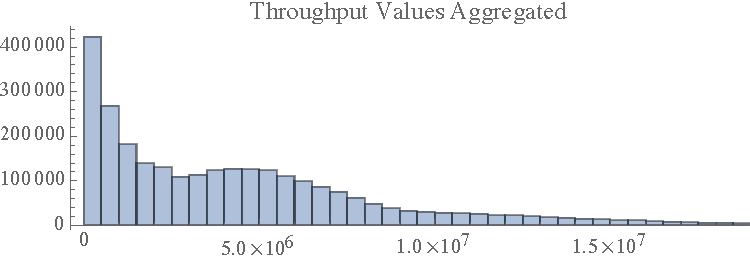
\includegraphics[width=.5\textwidth]{plot-histogram-throughput.pdf}
  \caption{Histogram of the raw throughput values recorded during all IOzone tests across all system configurations. The distribution is skewed right, with few tests having significantly higher throughput than most others.
  \vspace{-.5cm}}
  \label{fig:throughput_histogram}
\end{figure}

This paper presents a variability modeling case study with a five-dimensional dataset produced by executing the IOzone benchmark \cite{iozone} on a homogeneous cluster of computers. Each node contains two Intel Xeon E5-2637 CPUs offering a total of 16 CPU cores with 16GB of DRAM. While the CPU frequency varies depending on the test configuration, the I/O from IOzone is performed by an ext4 filesystem sitting above an Intel SSDSC2BA20 SSD drive. At the time of data collection, a Linux kernel version of 4.13.0 was used. The system performance data was collected over two weeks by executing IOzone 150 times for each of a select set of approximately 18K system configurations, for a total of approximately 2.7M executions of IOzone. A single IOzone execution reports the max I/O throughput in kilobytes per second seen for the selected test. The summary of the data generated in the experiments for this paper can be seen in Table \ref{tab:data_description}. Distributions of raw throughput values being modeled can be seen in Figure \ref{fig:throughput_histogram}.

Some mild preprocessing was necessary to prepare the data for modeling and analysis. All features were shifted by their minimum value and scaled by their range, mapping each feature independently into $[0,1]$. This normalization ensures each feature is treated equally by the interpolation techniques and should be performed on all data before building models and making predictions regardless of application. All 150 repeated trials for a system configuration were grouped with that configuration. The only non-ordinal feature in this data is the test. All tests were treated as different applications and were separated for modeling and analysis. (i.e. predictions for the ``readers'' test were made using known configurations for the ``readers'' test only.) The division of non-ordinal features into separate models is necessary for the presented methodology, however future improvements are discussed in Section \ref{sec:discussion}.

%% ===================================================================

\begin{figure}
  \begin{tikzpicture}
    \node (img)  {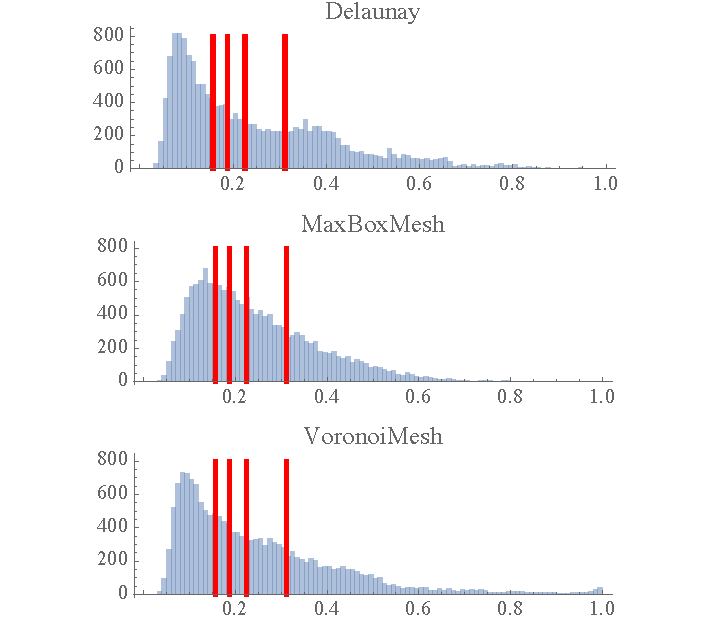
\includegraphics[width=0.5\textwidth,trim={1.5cm 0 0 0}]{plot-histogram-80_20-KS.pdf}};
    \node[below=of img, node distance=1cm, yshift=1cm] {KS Statistic for Predicted vs. Actual};
    \node[left=of img, node distance=0cm, rotate=90, anchor=center,yshift=-0.7cm] {Count};
  \end{tikzpicture}
  \caption{Histograms of the prediction error averaged over 10 folds for each modeling algorithm when trained with 80\% of the data. The distributions show the KS statistics for the predicted throughput distribution versus the actual throughput distribution. The four vertical red lines represent commonly used p-values \{0.05, 0.01, 0.001, 1.0e-6\} respectively. All predictions to the right of a red line represent failed predictions that are significantly different (by respective p-value) from the actual distribution according to the KS test.
  \vspace{-.1cm}}
  \label{fig:ks_histogram_80_20}
\end{figure}

\section{RESULTS}
\label{sec:results}

All three interpolation techniques are used to predict the distribution of I/O throughput values at previously unseen system configurations. In order to improve robustness of the error analysis, 10-fold cross validation is used. 10 random selections of 80\% of the IOzone data are used to train each model and the remaining 20\% provide estimations of approximation error for each model. The recorded errors are averaged over the 10 random folds and grouped by unique system configuration. The folds are identically seeded for each interpolation technique, ensuring consistency in the training and testing sets.

The aggregation of errors across all IOzone tests given 80\% of the data as training can be seen in Figure \ref{fig:ks_histogram_80_20}. Agglomerate errors for each technique present similarly, each resembles a Gamma distribution. The percentages of failed predictions with varying p-values are on display in Table \ref{tab:p_value_failure_rate}. The primary p-value used for analyses in this work is 0.001. This p-value is chosen because close to 2K predictions are made for each test. Also, applications executed in cloud and HPC systems that could benefit from statistical modeling will be executed at least on the order of 1000's of times. In line with this knowledge, it is important to ensure that only a small fraction of interpretable results could occur solely under the influence of random chance. When considering the p=0.001 results for each technique, a little under half of the generated predictions fail. In a traditional application of machine learning techniques a failure rate of 45\% would be a poor result, however in this situation the complexity of the problem warrants a slightly different interpretation. These predictions are of a very \textit{precise} characterization of performance variability, in fact the strongest possible characterization of variability. Globally, only a little under half of the predictions fail to capture \textit{all} of the characteristics of performance variability at new system configurations. It is also demonstrated later in this Section that this result can likely be improved.

\begin{table}
  \centering
  \begin{tabular}{c|c|c}
    \hline
    \textbf{Algorithm} & \textbf{P-Value} & \textbf{\% Failed Predictions} \\
    \hline
    \multilinecell{Delaunay\\Max Box Mesh\\Voronoi Mesh} & .05 & \multilinecell{58.4\\69.3\\61.9}\\
    \hline
    \multilinecell{Delaunay\\Max Box Mesh\\Voronoi Mesh} & .01 & \multilinecell{51.1\\58.4\\53.4}\\
    \hline
    \multilinecell{Delaunay\\Max Box Mesh\\Voronoi Mesh} & .001 & \multilinecell{44.1\\46.9\\45.1}\\
    \hline
    \multilinecell{Delaunay\\Max Box Mesh\\Voronoi Mesh} & 1.0e-6 & \multilinecell{31.4\\26.6\\28.7}\\
    \hline
  \end{tabular}
  \caption{The prediction failure rate by the KS-test when provided different selections of p-values. These accompany the results from Figure \ref{fig:ks_histogram_80_20}. 
    \vspace{-.5cm}}
  \label{tab:p_value_failure_rate}
\end{table}


While interpreting failure rates of these interpolation techniques, it is important to consider at what rate the error reduces with increasing amounts of training data. Figure \ref{fig:ks_failure_by_training} displays the change in p=0.001 failure rate with increasing density of training data up to the maximum density allowed by this training set. Delaunay provides the best results with the least training data by about 5\%, but these low-density prediction error rates are unacceptably high (90\% failure). Increased density demonstrates a roughly $(1 - \sqrt{n})$ rate of reduction in error that will level off around 20-30\% with a training set twice the size of the one collected for this study. However, constructing a training set of such a size would likely require months of compute time and be infeasible for many applications. The rate of convergence seen also suggests that these models are successfully converging on the lowest possible error given the (presumed) Lipschitz constant of the data and any latent variables that may perfectly describe system I/O throughput variability.

\begin{figure}
  \begin{tikzpicture}
    \node (img)  {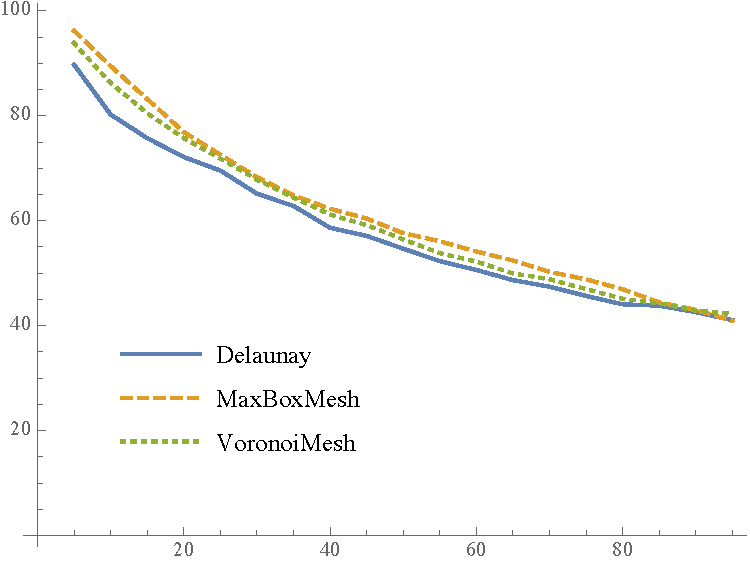
\includegraphics[width=0.4\textwidth,]{plot-KS-Failure-by-Training.pdf}};
    \node[below=of img, node distance=1cm, yshift=1cm] {Percentage of Training Data};
    \node[left=of img, node distance=0cm, rotate=90, anchor=center,yshift=-0.7cm] {Percentage of Failed Predictions};
  \end{tikzpicture}
  \caption{The performance of each algorithm with increasing amounts of training data estimated using 10-fold cross validation and the KS test with p=0.001. The KS statistic for any given training percentage is achieved by averaging over the KS statistic for all tests and system configurations. The training percentages range from 5\% to 95\% by increments of 5\%. Delaunay is the best performer until 95\% of data is used for training, at which Max Box mesh becomes the best performer by a fraction of a percent.
  \vspace{-.1cm}}
  \label{fig:ks_failure_by_training}
\end{figure}

It may be misleading to consider the global performance of each prediction technique across all tests, as some tests are more difficult than others to predict and have more apparent latent activity. In Figure \ref{fig:ks_failure_by_training_and_test}, the relative difficulty of each IOzone test can be compared. The I/O tests analyzing reads are typically approximated with lower error than those tests analyzing writes. Regardless of test, in the aggregate results the modal KS statistics hover consistently around 0.15, demonstrating an impressively low KS statistic for modal predictions. In order to address the opacity of aggregate analysis, another case study and an application of the methodology from Section \ref{sec:feature_weighting} is presented in Table \ref{tab:optimized_p_value_failure_rate}.

The results presented in Table \ref{tab:optimized_p_value_failure_rate} are achieved by permitting each approximation technique 300 iterations of modified simulated annealing. In each iteration, the impact of potential weights on average validation KS statistic were considered. All weights were kept in the range [0,2], and were applied to the normalized features for frequency, file size, record size, and number of threads. All three techniques converged on similar optimal weights for the validation sets of approximately \{.001, 2, 1.7, 1.5\} for each respective feature. Recall that each interpolation technique uses smaller distances to denote larger influence on predictions, meaning that frequency was the most important feature when predicting variability for the ``readers'' test, followed not-so-closely by number of threads, then record size.

The ``readers'' test results demonstrate that the underlying prediction techniques work and are capable of seeing failure rates below 5\% when optimized for a given application. It is important to emphasize that the roughly 95\% of predictions that did not fail are predicting the \textit{precise} distribution of I/O throughput that will be witnessed at a previously unseen system configuration. To present knowledge, there is no existing methodology that is generically applicable to any system performance metric, agnostic of system architecture, and capable of making such powerful predictions.

\begin{table}
  \centering
  \begin{tabular}{c|c|c|c}
    \hline
    \textbf{Algorithm} & \textbf{P-Value} & \multilinecell{\textbf{Unweighted}\\\textbf{\% Failure}} & \multilinecell{\textbf{Weighted}\\\textbf{\% Failure}}\\
    \hline
    \multilinecell{Delaunay\\Max Box Mesh\\Voronoi Mesh} & .05 & \multilinecell{24.9\\21.3\\18.7} & \multilinecell{30.2\\21.2\\11.3}\\
    \hline
    \multilinecell{Delaunay\\Max Box Mesh\\Voronoi Mesh} & .01 & \multilinecell{21.6\\16.4\\14.9} & \multilinecell{27.4\\16.4\\7.0}\\
    \hline
    \multilinecell{Delaunay\\Max Box Mesh\\Voronoi Mesh} & .001 & \multilinecell{19.7\\13.1\\12.3} & \multilinecell{25.4\\13.1\\4.6}\\
    \hline
    \multilinecell{Delaunay\\Max Box Mesh\\Voronoi Mesh} & 1.0e-6 & \multilinecell{17.9\\11.3\\8.5} & \multilinecell{23.4\\11.3\\2.3}\\
    \hline
  \end{tabular}
  \caption{The prediction failure rates by various p-values for the KS-test. These results are strictly for the ``readers'' IOzone test and show unweighted results as well as the results with weights optimized for minimum error (KS statistic) by 300 iterations of modified simulated annealing. Notice that the weights identified for the Delaunay model cause overfitting and reduction in apparent performance. MaxBoxMesh performance is improved by a negligible amount. VoronoiMesh predictions are notably improved.
    \vspace{-.5cm}}
  \label{tab:optimized_p_value_failure_rate}
\end{table}

%% \begin{itemize}
%% \item Case studies of good and bad predictions of distributions made, present 3 (best, median, worst)
%% \item Table / Figure showing error for each of the tests (hardest test to predict)
%% \item Presentation of the top most difficult configurations to predict for each test (and the bad performance at those points)
%% %% \item Comparison to predictions made using the "test" numerical column
%% \end{itemize}

\section{DISCUSSION}
\label{sec:discussion}

The results of the IOzone case study indicate that predicting the CDF of I/O throughput at previously unseen system configurations is a challenging problem. The KS statistic captures the worst part of any prediction and hence provides a conservatively large estimate of approximation error. The average absolute error in the predicted CDFs are always lower than the KS statistics. However, the KS statistic was chosen because of the important statistical theory surrounding it as an error measure. Considering this circumstance, a nonnegligible volume of predictions provide impressively low levels of error. Powerful predictive tools such as those presented in this work allow for more in-depth analysis of system performance variability. For example, system configurations that are most difficult to predict in these tests are likely ``outlier'' configurations that do not resemble those configurations that share many similar parameters. Analysis of these configurations may provide valuable insight into effective application specific operation of computer systems.

As mentioned in Section \ref{sec:introduction}, no prior work has attempted to model an arbitrary performance metric for a system to such a high degree of precision. All previous statistical modeling attempts capture few (\textless 3) ordinal measures of performance. Generating models that have such high degrees of accuracy allows system engineers to identify previously unused configurations that present desired characteristics. Service level agreements (SLAs) in cloud computing environments are cause for capital competition that is impacted heavily by system performance \cite{patel2009service}. Users prefer SLAs that allow the most computing power per capital expense, incentivizing service providers to guarantee the greatest possible performance. Overscheduling and irregular usage patterns force cloud service providers to occasionally overload machines, in which case precise models of system performance can be used to statistically minimize the probability of SLA violation. Similar targeted performance tuning techniques can be applied to HPC system configuration to maximize application throughput or minimize system power consumption.

A final application domain that may also be affected by this methodology is computer security. Collocated users on cloud systems are a source of recent attention \cite{ali2015security}. If a malicious collocated user is capable of achieving specific insight into the configuration of the system, or the activity of other collocated users by executing performance evaluation programs (i.e. IOzone), a new attack vector may present itself. Malicious users could be capable of identifying common performance distributions of vulnerable system configurations and vulnerable active user jobs. This knowledge may allow targeted exploits to be executed. Light inspection of raw IOzone I/O throughputs provides substantial evidence that distinct performance distributions coincide closely with specific system configuration parameters. Conversely, a service provider may defend against such attacks by deliberately obfuscating the performance of the machine. Models such as those presented in this paper could identify optimal staggering and time-delay whose introduction into the system would prevent malicious users from identifying system configurations and active jobs.


\begin{figure}
  \begin{tikzpicture}
    \node (img)  {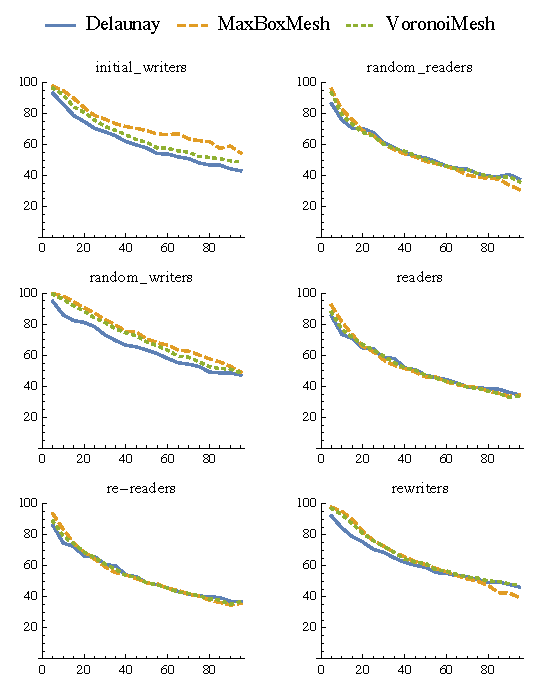
\includegraphics[width=0.4\textwidth,]{plot-KS-failure-by-training-and-test.pdf}};
    \node[below=of img, node distance=1cm, yshift=1cm] {Percentage of Training Data};
    \node[left=of img, node distance=0cm, rotate=90, anchor=center,yshift=-0.7cm] {Percentage of Failed Predictions};
  \end{tikzpicture}
  \caption{The performance of each algorithm on different IOzone tests with increasing amounts of training data measured using 10-fold cross validation and the KS test with p=0.001. The KS statistic for any given training percentage is achieved by averaging over the KS statistic for all tests and system configurations. The training percentages range from 5\% to 95\% by increments of 5\%. The ``readers'' tests tend to allow lower failure rates than the ``writers'' tests.
  \vspace{-.1cm}}
  \label{fig:ks_failure_by_training_and_test}
\end{figure}


It remains unclear what mathematical properties of each approximation technique contribute the most to overall accuracy. Results presented in Table \ref{tab:optimized_p_value_failure_rate} are particularly interesting, demonstrating that Delaunay appears most vulnerable to overfitting, Max Box mesh is largely invariant to feature scaling, and Voronoi mesh generalizes feature weights well to unseen configurations.

There are many avenues for extending this modeling methodology. One of the most severe limitations of the present framework is the restriction to modeling ordinal system parameters. Many applications have nonordinal settings and individually modeling all combinations of those settings is not a tractable solution. Automatic processing of categorical settings into an appropriate set of ordinal features constitutes future work. Presently the failure rate of distribution predictions can only be reduced with large volumes of performance data, however future work may be able to effectively reduce the amount of training data required by introducing appropriate expectations of stochastic noise in the measured performance. Finally, more case studies need to be explored in order to test the robustness of the present modeling techniques to changes in domain and performance metric.

\section{CONCLUSION}
\label{sec:conclusion}

The presented methodology and application is capable of providing new insights, extending existing analyses, and improving the management of computational performance variability. Each of Delaunay, Max Box, and Voronoi meshes are viable techniques for constructing approximations of performance cumulative distribution functions. A case study on I/O throughput demonstrated that models are capable of effectively predicting most unseen system configurations for any of the available I/O tests. The present methodology represents a notable increase in the ability to statistically model arbitrary system performance metrics involving the interaction of many ordinal system parameters.
%% \begin{itemize}
%% \item Modeling the distributions of system performance is valuable.
%% \item This work presents a steep increase in the power of predictions made by statistical modeling techniques.
%% \end{itemize}

\bibliographystyle{IEEEtran}
\bibliography{paper}

\end{document}
